\documentclass{article}
\usepackage{amsfonts} % \mathbb
\usepackage[margin=0.5in]{geometry}
\usepackage[utf8]{inputenc}
\usepackage{graphicx} 

\title{Interference Transform: Estimating the frequency and phase of low resolution samples}
\author{
  Carlos Tarjano
  \and 
  Valdecy Pereira
  }

\begin{document}

\maketitle

\begin{abstract} % 250 words
  % background
  The Fourier Transform, naturally due to the context and time in which it was idealized, was formulated without regard to discrete waves or computational complexity.
  Some developments, such as the Discrete Fourier Transform and the Fast Fourier Transform algorithm updated the theory to the digital, discrete era.
  % motivation
  A meaningful,
  % objective
  In this paper we propose a formal framework based on discrete waves, optimizing the inference of frequency and amplitude from whatever sampled points are available. Although arising from a intuitively different approach, the framework here presented can be viewed as a generalization of the Discrete Fourier Transform.
  % methods
  The algorithm is based on the representation of the set of samples in a frequency versus phase space and the investigation of the interference pattern thus generated. Each sample defines a sinusoidal planar wave in this space, with a particular amplitude, direction and frequency. The determination of the point in which maximum constructive interference occurs translates to the determination of the most accurate sinusoidal description of the whole set of samples.
  % results
  % TODO: improvement of the naïve algorithm. better accuracy
  % implications
  % TODO: an alternative to wavelet and short-time Fourier transform
\end{abstract}

{\bf Keywords:} Signal Representation, Audio Compression,

\section{Introduction}

\subsection{Literature Review}

\section{Methodology}

\subsection{Theory}

  \begin{figure}[h!]
    \centering
      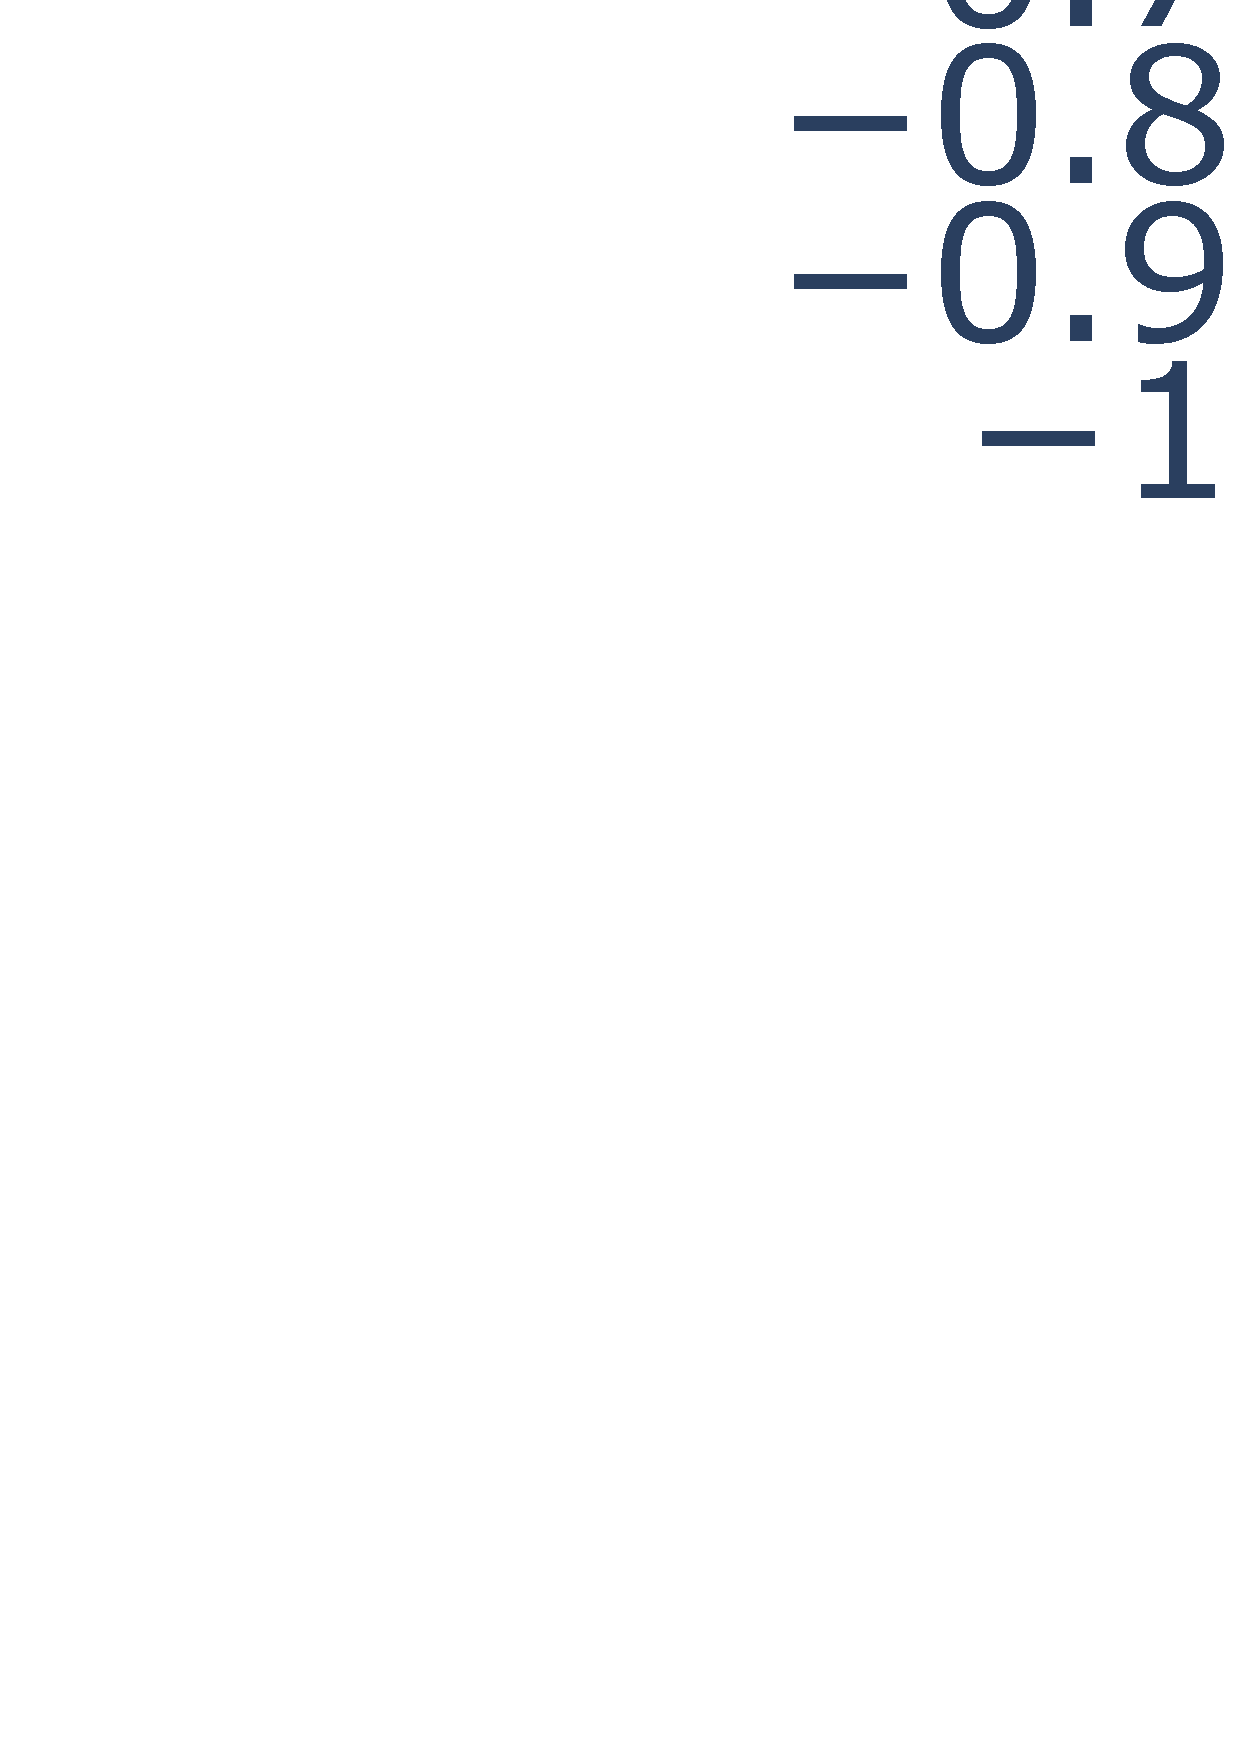
\includegraphics[width=0.8\linewidth]{images/01ContinuousVsDiscrete.pdf}
    \caption{Discrete samples (black points) from a continuous wave (grey line). Note that the amplitude is also truncated}
    \label{fig:ContinuousVsDiscrete}
  \end{figure}
  
\section{Results}

\section{Discussion + Conclusion}

\section{References}

\end{document}
